% 2003 年江苏卷第 19 题：直三棱柱立体几何图
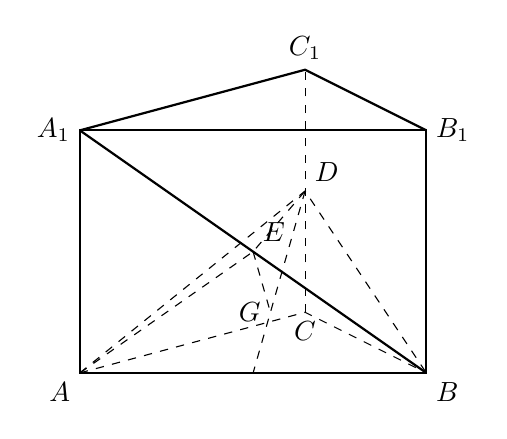
\begin{tikzpicture}[>=stealth,scale=1.1]
  % Vertices
  \coordinate (A) at (0,0);
  \coordinate (B) at (4,0);
  \coordinate (A1) at (0,2.8);
  \coordinate (B1) at (4,2.8);
  \coordinate (C) at (2.6,0.7);
  \coordinate (C1) at (2.6,3.5);
  
  \coordinate (D) at (2.6,2.1); % midpoint of CC1
  \coordinate (E) at (2,1.4);   % midpoint of A1B
  
  \coordinate (M) at (2,0);     % midpoint of AB
  \coordinate (G) at (2.2,0.7); % centroid of ABD on median DM
  
  % Solid visible edges of prism
  \draw[thick] (A) -- (B) -- (B1) -- (A1) -- cycle;
  \draw[thick] (A1) -- (C1) -- (B1);
  \draw[thick] (A1) -- (B); % diagonal
  
  % Dashed edges of prism
  \draw[dashed] (A) -- (C) -- (B);
  \draw[dashed] (C) -- (D) -- (C1);
  
  % Dashed lines for problem geometry
  \draw[dashed] (A) -- (D) -- (B);
  \draw[dashed] (A) -- (E) -- (D);
  \draw[dashed] (E) -- (G);
  \draw[dashed] (D) -- (M);
  
  % Labels
  \node[below left] at (A) {$A$};
  \node[below right] at (B) {$B$};
  \node[left] at (A1) {$A_1$};
  \node[right] at (B1) {$B_1$};
  \node[below] at (C) {$C$};
  \node[above] at (C1) {$C_1$};
  \node[above right] at (D) {$D$};
  \node[above right] at (E) {$E$};
  \node[left] at (G) {$G$};
\end{tikzpicture}
